\documentclass{beamer}
 
\usepackage[utf8]{inputenc}
\usepackage{amsmath}
\usepackage{amssymb}
\usepackage{esint}
% \usepackage{physics}

\renewcommand\mathfamilydefault{\rmdefault}
 
 
%Information to be included in the title page:
\title{Electromagnetic Waves Math}
\author{Ben Kettle}
\date{16 Jan 2020}
 
\begin{document}
 
\frame{\titlepage}

\begin{frame}{Maxwell's Equations}
    \begin{columns}
    \begin{column}{0.5\textwidth}
        \begin{center}
            Gauss's Law for $\vec{\mathbf{E}}$
        \end{center}
       \[ \oiint_S \vec{\mathbf{E}}\cdot d\vec{\mathbf{A}} = \frac{Q}{\varepsilon_0} \]
       Electric  flux  through  a  closed  surfaceis proportional to the charged enclosed
       \end{column}
       \begin{column}{0.5\textwidth}
        \begin{center}
            Faraday's Law
        \end{center}
        \[ \oint \vec{\mathbf{E}}\cdot d\vec{\mathbf{s}} = -\frac{d\Phi_B}{dt}\]
        Changing  magnetic  flux  produces  an  electric field 
    \end{column}
    \end{columns}
    
    \begin{columns}
    \begin{column}{0.5\textwidth}
        \begin{center}
            Gauss's Law for $\vec{\mathbf{B}}$
        \end{center}
       \[ \oiint_S \vec{\mathbf{B}}\cdot d\vec{\mathbf{A}} = 0 \]
       The   total   magnetic   flux   through   a closed surface is zero 
       \end{column}
       \begin{column}{0.5\textwidth}
        \begin{center}
            Ampere-Maxwell Law
        \end{center}
        \[ \oint \vec{\mathbf{B}}\cdot d\vec{\mathbf{s}} = \mu_0 I + \mu_0\varepsilon_0\frac{d\Phi_E}{dt}\]
        Electric  current  and  changing  electric  flux produces a magnetic field
    \end{column}
    \end{columns}
\end{frame}

\begin{frame}{Maxwell's Equations in Empty Space}
    When we assume $Q=0$ and $I=0$, as is the case for travelling electromagnetic waves, these get a bit simpler:
    \begin{columns}
    \begin{column}{0.5\textwidth}
        \begin{center}
            Gauss's Law for $\vec{\mathbf{E}}$
        \end{center}
       \[ \oiint_S \vec{\mathbf{E}}\cdot d\vec{\mathbf{A}} = 0 \]
        \begin{center}
            Faraday's Law
        \end{center}
        \[ \oint \vec{\mathbf{E}}\cdot d\vec{\mathbf{s}} = -\frac{d\Phi_B}{dt}\]
    \end{column}
    
    \begin{column}{0.5\textwidth}
        \begin{center}
            Gauss's Law for $\vec{\mathbf{B}}$
        \end{center}
       \[ \oiint_S \vec{\mathbf{B}}\cdot d\vec{\mathbf{A}} = 0 \]
        \begin{center}
            Ampere-Maxwell Law
        \end{center}
        \[ \oint \vec{\mathbf{B}}\cdot d\vec{\mathbf{s}} = \mu_0\varepsilon_0\frac{d\Phi_E}{dt}\]
    \end{column}
    \end{columns}
\end{frame}

\begin{frame}{EM Wave Basics}
    A key fact for electromagnetic waves is that they are \alert{transverse}---both the $\vec{E}$ and $\vec{B}$ fields are perpendicular to the direction of propagation. The fields are also perpendicular to each other, so where $\vec{\mathbf{p}}$ is the direction of propagation:
    \[ \vec{\mathbf{E}} \times \vec{\mathbf{B}} = \vec{\mathbf{p}} \]
    
\end{frame}

\begin{frame}{The Wave Equation for EM waves}
    Our goal is to find the \alert{wave equation} for the EM wave---something of the form:
    \[ \left(\frac{\partial^2}{\partial x^2}-\frac{1}{v^2}\frac{\partial^2}{\partial t^2}\right)\psi(x,t)=0 \]
    
    Where $\psi(x,t)$ is the wave function itself and $v$ is the wave velocity. To do this, we will apply Faraday's Equation and the Ampere-Maxwell law to an electromagnetic wave. 
    
\end{frame}

\begin{frame}{The Wave Equation for EM waves}
    \begin{columns}
    \begin{column}{.5\textwidth}
    Setting our coordinate system such that the $\vec{E}$ field is in the $xy$ plane and the $\vec{B}$ field is in the $xz$ plane, the wave equation for an electromagnetic wave can be found using multivariable calcalculus. \vspace{2mm}
    
    Using the Faraday Equation, we can integrate over a loop in the $xy$ plane to find:
    \[ \frac{\partial E_y}{\partial x} = -\frac{\partial B_z}{\partial t} \]
    \end{column}
    \begin{column}{.5\textwidth}
        \begin{figure}
            \centering
            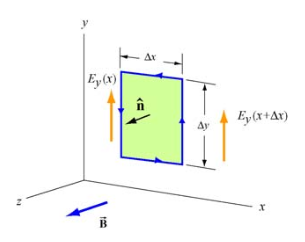
\includegraphics[scale=.8]{efieldint.png}
            \caption{Applying Faraday's Law to a loop in the $xy$ plane.}
            \label{fig:my_label}
        \end{figure}
    \end{column}
    \end{columns}
\end{frame}

\begin{frame}{The Wave Equation for EM waves}
    Then, following the same steps with Ampere-Maxwell and a loop in the $xz$ plane, we reach:
    \[ - \frac{\partial B_z}{\partial x} = \mu_0\varepsilon_0\frac{\partial E_z}{\partial t}\]
    \begin{figure}
        \centering
        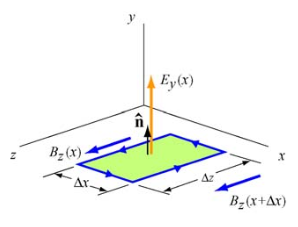
\includegraphics[scale=.9]{bfieldint.png}
        \caption{Applying Ampere-Maxwell to a loop in the $xz$ plane.}
        \label{fig:my_label}
    \end{figure}
\end{frame}

\begin{frame}{Velocity of an EM Wave}
    The equation describing any wave is given in a general form of:

    \[ \left(\frac{\partial^2}{\partial x^2}-\frac{1}{v^2}\frac{\partial^2}{\partial t^2}\right)\psi(x,t)=0 \]
    Where $\psi(x,t)$ is the wave function itself and $v$ is the wave velocity. More manipulation of the two equations from the last sides yields us something in a similar format:
    \[  \left(\frac{\partial^2}{\partial x^2}-\mu_0\varepsilon_0\frac{\partial^2}{\partial t^2}\right)\left\{ \begin{array}{c} E(x,t) \\ B(x,t) \end{array} \right\}=0 \]

    We can then clearly find the velocity of an electromagnetic wave:
    \[ \frac{1}{v^2} = \mu_0\varepsilon_0 \longrightarrow v = \frac{1}{\sqrt{\mu_0\varepsilon_0}}\]
\end{frame}

\begin{frame}{Proving that light is an EM wave}
    We can use this fact to show that light is an example of an electromagnetic wave.
    
    \[ v=\frac{1}{\sqrt{\mu_{0} \varepsilon_{0}}}=\frac{1}{\sqrt{\left(4 \pi \times 10^{-7} T \cdot m/A\right)\left(8.85 \times 10^{-12} C^{2} / N \cdot m^{2}\right)}} \] 
    \[ v =2.997 \times 10^{8} m/s=c \]
\end{frame}

\begin{frame}{More EM Wave Properties}
    Had we done the full derivation of the above fact, we would also be able to show that:
    \[ \frac{E}{B} = c \] 
    This means that in an electromagnetic wave, the $\vec{E}$ field is much larger than the $\vec{B}$ field.
\end{frame}

\begin{frame}{Summary: The Important Slide}
    That was probably confusing. So to summarize what we know:
    \begin{itemize}
	\item The wave is transverse because $\vec{E}$ and $\vec{B}$ are perpendicular to the direction of propagation $\vec{p}$, which is given by $\vec{p} = \vec{E} \times \vec{B}$.
	\item The $E$ and $B$ fields are perpendicular to each other, meaning $\vec{E} \cdot \vec{B} = 0$.
	\item $\frac{E}{B} = \frac{E_0}{B_0} = c$
	\item The wave's speed of propagation equals $\frac{1}{\sqrt{\mu_0\epsilon_0}}$
	\item The superposition principle applies to the waves---two overlapping waves can be added to give the resulting wave.
    \end{itemize}
\end{frame}

\end{document}